\documentclass[12pt, a4paper,usenames,dvipsnames]{article}
\usepackage[utf8]{inputenc}
\usepackage[english]{babel}
\usepackage{amsmath,amssymb,amsthm} 
\usepackage{graphicx}
\usepackage{siunitx}
    \sisetup{exponent-product = \cdot} 
    \sisetup{separate-uncertainty = true}
\usepackage[margin=20mm, tmargin=30mm,headheight=15pt ]{geometry}
\usepackage{fancyhdr}
\usepackage{framed}
\usepackage{caption}
\usepackage{subcaption}
\usepackage{lastpage}  
\pagestyle{fancy}
    \fancyhf{}
    \rhead{Endre Sørmo Rundsveen}
    \lhead{Assignment 1 - MA2501}
    \rfoot{Page \thepage \ of \pageref{LastPage}}
\usepackage{tikz}
\usetikzlibrary{calc}
\usetikzlibrary{patterns}
\usepackage{lettrine}
\title{Assignment 2 - MA2501}
\author{Endre Sørmo Rundsveen}
\usepackage{sectsty}
\usepackage{bm}
\sectionfont{\color{Mahogany}}
\subsectionfont{\color{Mahogany}}

\usepackage{listings}%Code show
\lstdefinestyle{mystyle}{
    backgroundcolor=\color{Aquamarine!1},
    commentstyle=\color{YellowGreen},
    keywordstyle=\color{Mahogany}\bfseries,
    numberstyle=\tiny,
    stringstyle=\color{OliveGreen},
    basicstyle=\footnotesize,
    breakatwhitespace=false,         
    breaklines=true,                 
    captionpos=t,                    
    keepspaces=true,                 
    numbers=left,                    
    numbersep=1pt,                  
    showspaces=false,                
    showstringspaces=false,
    showtabs=false,                  
    tabsize=1,
    xleftmargin=0.5em,
    frame=topline
}
 
\lstset{style=mystyle}
\renewcommand\vec{\mathbf}
\begin{document}

\begin{titlepage}
    \newgeometry{tmargin=125mm}
    \begin{tikzpicture}[remember picture,overlay]
        \fill[Aquamarine!10] ($(current page.south west)+(0cm,15cm)$) rectangle (current page.north east);
    \end{tikzpicture}
  \centering
    {\noindent \Huge \color{Brown}{\underline{Assignment 2 - MA2501}}}\\
    
    {\large \color{Brown}{Endre Sørmo Rundsveen}}\\
    \raggedright
    \hfill \break
    \lettrine[lraise=0.15]{T}{} he following document are my solution to the second assignment of MA2501 in the spring semester of 2019. Throughout one can assume that the packages \textit{sympy, numpy,} and \textit{matplotlib}, are imported as follows
    \begin{lstlisting}[language=Python]
    import matplotlib
    import matplotlib.pyplot as plt
    import numpy as np
    import sumpy as symp\end{lstlisting}
\end{titlepage}
\restoregeometry
\twocolumn

\section*{Problem 1}
\subsection*{(a)}
In the following the Newton method is going to be implemented to approximate the solution of nonlinear functions in two variables. The Newton method is a fixed point iteration which for \[\left\{\begin{array}{l}
    F:\mathbb{R}^2\rightarrow \mathbb{R}^2   \\
    (x_1,x_2)\mapsto (f_1(x_1,x_2),f_2(x_1,x_2)) 
\end{array}\right.\] is defined as
\begin{equation*}
    G(x^{(k)})=x^{(k)}-J(x^{(k)})^{-1}F(x^{(k)})
\end{equation*}
where the \textit{Jacobian} is the matrix function
\[J(x)=\left(\begin{array}{cc}
     \frac{\partial f_1}{\partial x_1}(x)& \frac{\partial f_1}{\partial x_2}(x) \\
     \frac{\partial f_2}{\partial x_1}(x)&\frac{\partial f_2}{\partial x_2}(x) 
\end{array}\right)\]
Beside of the singularity check, have I in the implementation opted to use the function \textit{lambdify} in the \textit{sympy} library over the \textit{subs} function. This should be a faster function and the output is automatically in float representation. With \textit{subs}, the output remained in symbolic representation. 
\begin{lstlisting}[language=Python]
def Newt(F,x0,N,Tol):
    #F is a vector function in two dim, with the variables x1 and x2.
    #x0 is the starting point
    #N is the maximum iterations
    #Tol is the tolerance of the approximation
    J=F.jacobian([x1,x2])
    if (J.subs({x1:x0[0],x2:x0[1]})).det()==0: #This method only works if the jacobian is nonsingular in a neighbourhood of x0
        return 
    invJ=symp.lambdify((x1,x2),J.inv(),"numpy")
    Fx=symp.lambdify((x1,x2),F.T,"numpy")#need to transpose F to make the dimensions for multiplication right
    i=0
    x01=x0
    xresult=[x01]
    Fx01=Fx(x01[0],x01[1])
    while i<N:
        x01=x01-invJ(x01[0],x01[1]).dot(Fx01[0])
        xresult.append(x01)
        Fx01=Fx(x01[0],x01[1])
        if np.linalg.norm(Fx01)<Tol or np.linalg.norm(xresult[i+1]-xresult[i])<Tol:
            return xresult
        i+=1
    return xresult
\end{lstlisting}
\subsection*{(b)}
Further the method was used to solve \(F(x)=0\) when
\[f_1(x_1,x_2)=x_1^2+x_2^2-2, \quad f_2=x_1-x_2,\]
by running the following code and repling the values on line 3 to start where you want.
\begin{lstlisting}[language=Python]
x1,x2=symp.symbols('x1,x2')
F=symp.Matrix([x1**2+x2**2-2,x1-x2])
x0=np.array([0,1])#Exchange values for the starting point of your choice
print(Newt(F,x0,100,10**(-7)))
\end{lstlisting}
In table \ref{tab:outNewt} I have listed the output for a few different \((x_1^{(0)},x_2^{(0)})^T\).

\begin{table}[h!]
    \centering
    \begin{tabular}{ll}
        Start & Output  \\ \hline
        \((0,1)\) &\((1,1)\)\\
        \((1,0)\)&\((1,1)\)\\
        \((-1,0)\)&\((-1,-1)\)\\
        \((0,-1)\)&\((-1,-1)\)\\
        \((0,-10)\)&\((-1,-1)\)\\
        \((0,10)\)&\((1,1)\)\\
        \((10,0)\)&\((1,1)\)\\
        \((-10,0)\)&\((-1,-1)\)
    \end{tabular}
    \caption{Output of newtons method for different starting points}
    \label{tab:outNewt}
\end{table}
These results should stand as a verification that whenever \(x_1^{(0)}+x_2^{(0)}<0\) the method converges to \((-1,-1)\) and whenever \(x_1^{(0)}+x_2^{(0)}>0\) the method converges to \((1,1)\)
\subsubsection*{Convergence}
To verify the quadratic convergence of the method we are to look at eq. \ref{eq1}, and verify that it converges to an value. 
\begin{equation}
    \lim_{k\to\infty}\frac{\|x^{(k+2)}-x^{(k+1)}\|_2}{\|x^{(k+1)}-x^{(k)}\|_2^2}
    \label{eq1}
\end{equation}
\begin{table}[h!]
    \centering
    \begin{tabular}{cc}
        Iteration & \(\frac{\|x^{(k+2)}-x^{(k+1)}\|_2}{\|x^{(k+1)}-x^{(k)}\|_2^2}\)  \\ \hline
        1&0.06932419423397524\\
        2&0.13351516416332435\\
        3&0.23370199508176395\\
        4&0.32527890768433959\\
        5&0.35232878408745028\\
        6&0.35355126238992807
    \end{tabular}
    \caption{Table showing the quadratic convergence.}
    \label{tab:quadconv}
\end{table}

\noindent We can see by table \ref{tab:quadconv} that the limit seems to be approximately \(0.354\), and thus the method converges quadratically.\\
In figure \ref{fig:x1x2pos} and \ref{fig:x1x2neg}, you can tell that \(x_1^{(k)}=x_2^{(k)}\) for increasing \(k\) for both possible limits.

\begin{figure}
    \centering
    \includegraphics[width=\linewidth]{x1x2.png}
    \caption{Plot of \(x_1^{(k)}\) and \(x_2^{(k)}\), showing that they converges to \(x_1^{(k)}=x_2^{(k)}=1\) for \(x_1^{(0)}+x_2^{(o)}>0\)}
    \label{fig:x1x2pos}
\end{figure}
\begin{figure}
    \centering
    \includegraphics[width=\linewidth]{x1x2neg.png}
    \caption{Plot of \(x_1^{(k)}\) and \(x_2^{(k)}\), showing that they converges to \(x_1^{(k)}=x_2^{(k)}=-1\) for \(x_1^{(0)}+x_2^{(o)}<0\)}
    \label{fig:x1x2neg}
\end{figure}

In figure \ref{fig:Fx} and \ref{fig:xfollow}, the norms \(\|F(x^{(k)}\|_2\) and \(\|x^{(k+1)}-x^{(k)}\|_2\) are plotted versus the number of iterations.
\begin{figure}
    \centering
    \includegraphics[width=\linewidth]{Fx.png}
    \caption{Plot of \(\|F(x^{(k)}\|_2\) versus the number of iterations}
    \label{fig:Fx}
\end{figure}
\begin{figure}
    \centering
    \includegraphics[width=\linewidth]{xfollow.png}
    \caption{Plot of \(\|x^{(k+1)}-x^{(k)}\|_2\) versus the number of iterations}
    \label{fig:xfollow}
\end{figure}



\newpage
\section*{Problem 2}
Problem 2 tasks us to implement three different methods of solving the linear system
\[A\Vec{u}=\Vec{f}\]
where \(A=(L+\Delta x^2k^2I_{n^2\times n^2})\in \mathbb{R}^{n^2\times n^2}\), \(k\in\mathbb{R}\), \(\Delta x=\frac{1}{n}\), \(\Vec{f}\in\mathbb{R}^{n^2}\),
\[L=\left(\begin{array}{ccccc}
     B&I_n&&&0  \\
     I_n&\ddots&\ddots&&\\
     &\ddots&\ddots&\ddots&\\
     &&\ddots&\ddots&I_n\\
     0&&&I_n&B
\end{array}\right),\]
where 
\[B=\left(\begin{array}{ccccc}
     4&1&&&0  \\
     1&\ddots&\ddots&&\\
     &\ddots&\ddots&\ddots&\\
     &&\ddots&\ddots&1\\
     0&&&1&4
\end{array}\right)\in\mathbb{R}^{n\times n}.\]
This is a linear system arising from the dicretization of the Helmholtz partial differential equation on the unit square \(\Omega=[0,1]\times [0,1]\) (see figure \ref{fig:omega}). The code for matrix \(A\) was given, and is thus not reproduced in this report.

\begin{figure}[h!]
    \centering
    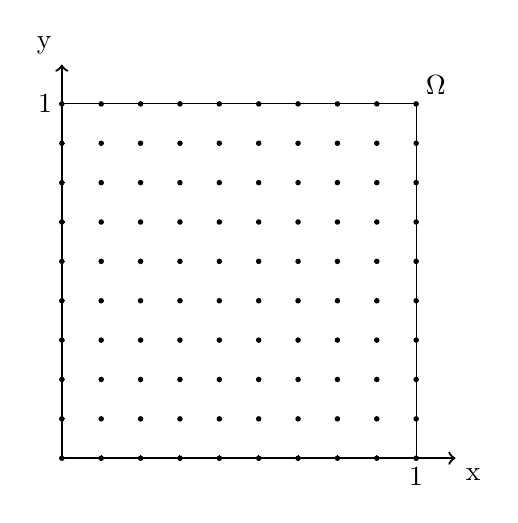
\begin{tikzpicture}
    \draw[thick,->] (0,0) -- (5,0) node[anchor=north west] {x};
    \draw[thick,->] (0,0) -- (0,5) node[anchor=south east] {y};
    \foreach \x in {0,0.5,1,1.5,2,2.5,3,3.5,4,4.5}
        \draw (\x cm,1pt) -- (\x cm,-1pt);
    \foreach \y in {0,0.5,1,1.5,2,2.5,3,3.5,4,4.5}
        \draw (1pt,\y cm) -- (-1pt,\y cm);
    \foreach \x in {0,0.5,1,1.5,2,2.5,3,3.5,4,4.5}
        \foreach \y in {0,0.5,1,1.5,2,2.5,3,3.5,4,4.5}
            \fill[color=black] (\x,\y) circle (1pt);
    \draw[thin](4.5,0)node[anchor=north]{1}--(4.5,4.5)node[anchor=south west]{\(\Omega\)}--(0,4.5)node[anchor=east]{1};        
    \end{tikzpicture}
    \caption{Discretization of the unit square}
    \label{fig:omega}
\end{figure}
The function
\[f=\exp{(-50(\left(x-\frac{1}{2}\right)^2+\left(y-\frac{1}{2}\right)^2))}\]
restricted to the domain \(\Omega\) gives the elements of \(\Vec{f}\) by \(f_l:=f(x_i,y_i)\), where \(l= (j-1) n + i\in\{1,2,...,n^2\}\), and \(x_i=\Delta x\cdot i,y_j=\Delta x\cdot j\). As a feature of how the task was presented, we iterate \(i,j\) over \([1,n]\), since else the dimensions would not coincide. Listing \ref{lst:omegafunc} shows the dicretization of the domain and the making of \(\Vec{f}\) over this discretization.
\begin{lstlisting}[language=python,caption=The discretization of \(\Omega\) and the making of \(\Vec{f}\),label=lst:omegafunc]
import scipy.sparse as scsp
def fl(x,y):#The elementfunctions of the vectorfunction
    return np.exp(-50*((x-1/2)**2+(y-1/2)**2))
def xiyi(n):
    #All the different x_i and y_i, starting with the first horizontal column
    l=[]
    #starting from (1,1) because otherwise we would get (n+1)x(n+1) matrices
    for i in range(1,n+1):
        for j in range(1,n+1):
            l.append([(1./n)*i,(1./n)*j])
    return l
l=xiyi(n)
F=np.array([fl(l[i][0],l[i][1]) for i in range(len(l))])
\end{lstlisting}
The solution of the aforementioned linear system are to be done using three different iterations method of the type
\[\vec{u}^{(k+1)}=A_1^{-1}(A_2\vec{u}^{(k)}+\vec{f})\]
where \(A=A_1-A_2\) and \(|A_1|\not=0\). \(A_1\) and \(A_2\) are found in the following way for the respective methods
\begin{itemize}
    \item Jacobi, \(A_1=A_d\)
    \item Forward Gauss-Seidel, \(A_1=A_d+A_l\)
    \item Successive over relaxation, \(A_1=A_d+\omega A_l\) (\(\omega\) is to be choosen by me)
\end{itemize}
By observing that all of these can be rewritten as 
\begin{itemize}
    \item Jacobi, \(A_1=A_d+\omega A_l\) with \(\omega=0\)
    \item Forward Gauss-Seidel, \(A_1=A_d+\omega A_l\) with \(\omega=1\)
    \item Successive over relaxation, \(A_1=A_d+\omega A_l\) 
\end{itemize}
The code can be written more compact. Further in the problem, we will need the spectral radius of \(A_1^{-1}A_2\), so the following code (Listing \ref{lst:iter}) also outputs this.
\begin{lstlisting}[language=python,caption=The function implementing the iterative methods.,label=lst:iter]
def LinearIter(A,u0,F,N=1000,omega=0,Tol=1e-7):
    #Omega = 0 gives Jacobi, omega = 1 gives Gauss-Seidel, 
    #omega = appropriate value gives SOR
    A_1=(scsp.diags(A.diagonal())+omega*scsp.tril(A,k=-1)).toarray()
    A_2=A_1-A.toarray()
    #Converting the matrices to array lets me use numpy to invert the matrix
    A_1inv=np.linalg.inv(A_1)
    def iteration(A_1inv,A_2,u_k,f):
        return A_1inv.dot(A_2.dot(u_k)+f)
    i=0
    r=[F-A.dot(u0)] #List of residuals
    u=u0 #List of consecutive approximations to x for Ax=F
    while i<N:
        u= iteration(A_1inv,A_2,u,F)
        r.append(F-A.dot(u))
        i+=1
        if np.linalg.norm(r[i])<Tol:
            break
    #The spectral radius of the matrix
    spec=np.amax(np.absolute(np.linalg.eigvals(A_1inv.dot(A_2))))
    return u,r,spec
\end{lstlisting}

Since no other vector is given I will run the code with \(\vec{u}^{(0)}=(0,0,\cdots,0)^T\).
\subsubsection*{Minimizing the spectral radius}
It was hinted that a lower spectral radius of \(A_1^{-1}A_2\), would give a positive effect to the convergence rate of the methods, so in an effort to make SOR the fastest of the method, I tried to minimize the spectral radius over \(\omega\). Using the following coe (Listing \ref{lst:omegaFind}), the figure \ref{fig:spec} shows the plot of  \(\rho(A_1^{-1}A_2)\) for \(\omega \in [-100,100]\).
\begin{lstlisting}[language=python,caption=Minimizing \(\rho(A_1^{-1}A_2)\) over \(\omega\).,label=lst:omegaFind]
rolist=[]
def ro(A,omega):
    A_1=(scsp.diags(A.diagonal())+omega*scsp.tril(A,k=-1)).toarray()
    A_2=A_1-A.toarray()
    A_1inv=np.linalg.inv(A_1)
    return specRad((A_1inv.dot(A_2)))
for i in np.linspace(-100,100,2000):
    rolist.append((ro(A,i),i))
om=min(rolist, key=lambda tup:tup[0])
\end{lstlisting}
\begin{figure}[h!]
    \centering
    \includegraphics[width=\linewidth]{ro.png}
    \caption{Plot of the spectral radius with a minimum for \(\omega=1.5507753876938466\), where \(\rho(A_1^{-1}A_2)=0.7639732791353856\).}
    \label{fig:spec}
\end{figure}
\subsubsection*{Plots}
In figure \ref{fig:res} one can observe that the residual for the SOR-method goes towards zero faster than the other methods. In the table \ref{tab:Specrad}, the spectral radius of each method are given. In dual, the table and graph, suggests that there are something to the aforementioned claim about convergence and spectral radius.
\begin{table}[h!]
    \centering
    \begin{tabular}{ll}
        \(\omega\) & \(\rho(A_1^{-1}A_2)\)  \\ \hline
        0 &0.95949321348780192\\
        1&0.92062722672914532\\
        1.55&0.7639732791353856
        
    \end{tabular}
    \caption{\(\omega\) and the associated spectral radius}
    \label{tab:Specrad}
\end{table}
\begin{figure}[h!]
    \centering
    \includegraphics[width=\linewidth]{2a.png}
    \caption{Plot of the residual for each method}
    \label{fig:res}
\end{figure}

\noindent Plotting (figure \ref{fig:specres}) the residual of each method and \(\|r^{(0)}\|_2\rho^k\) (where \(\rho\) is the spectral radius) further suggests a close relationship between the convergence and spectral radius.
\begin{figure}[h!]
    \centering
    \includegraphics[width=\linewidth]{2b.png}
    \caption{Plot giving evidence to relation between convergence and spectral radius}
    \label{fig:specres}
\end{figure}
\subsubsection*{Relative time}
In my endeavour to find the time used of each methods I first used the library \textit{time} and the function \textit{time.timeit()}, but this gave an output time which fluctuated from each time the function were called, most likely since this were dependent on what other programs which were running at the time. Thus I opted to use the library \textit{timeit} and the function \textit{timeit.timeit()}, which ran the code several time to reduce the local fluctuations. Table \ref{tab:time} gives these respective times. Showing that the SOR-method are the fastest, followed by Gauss-Seidel and Jacobi.
\begin{table}[h!]
    \centering
    \begin{tabular}{lr}
        \(\omega\) & Time (\(s\))  \\ \hline
        0 &16.955462826666917\\
        1&11.20701141333484\\
        1.55&6.925723306667351
        
    \end{tabular}
    \caption{\(\omega\) and the associated time used to run the method 1000 times.}
    \label{tab:time}
\end{table}
\subsubsection*{Relation between \(k\) and \(\Delta x\)}
The lack of time forces me to only give a small comment on how the wave number and step size relates to each other. One can see that if the step size (\(\Delta x)\) is held constant and the wave number increases, the values on the diagonal increases. Further the size of the eigenvalues of a matrix is very affected by the diagonal, so that higher values on the diagonal gives higher eigenvalues. Since \(A_1^{-1}A_2\) has smaller values on the diagonal when k increases, this would suggest that for higher wave numbers, the convergence gets more rapid.
\end{document}
